\documentclass[../Cover.tex]{subfiles}

\begin{document}
	\begin{minipage}[t][0.2\textheight][t]{0.1\textwidth} 
		\includegraphics[width=\textwidth]{\logo}
	\end{minipage}
	\hfill
	\begin{minipage}[t][0.2\textheight][t]{0.8\textwidth}
		\begin{tabular}{ p{0.25\textwidth} l  }		
			\\	
			\small \textbf{1 to 5 Carbine Drill} \\
			\\[0.09\textheight]
		\end{tabular}
		\quad
		%%%%%%%%%%%%%%%%%%%%%%%%%%%
		% Quick Facts Table       %
		%%%%%%%%%%%%%%%%%%%%%%%%%%%
		\begin{tabular}{ | p{0.2\textwidth} | p{0.2\textwidth} | p{0.1\textwidth} |}
			\hline
			\rowcolor[HTML]{C0C0C0}\tiny Weapon Type & \tiny Distance & \tiny Par Time\\ 
			\hline
			\tiny Rifle & \tiny 5yd & \tiny 5s \\ % EDIT HERE
			\hline
		\end{tabular}
	\end{minipage}
	%%%%%%%%%%%%%%%%%%%%%%%%%%%
	% Requirements      %
	%%%%%%%%%%%%%%%%%%%%%%%%%%%
	\begin{tabular}{p{0.25\textwidth}}
		\small Requirements \\
		\hline
		\tiny \begin{itemize} % EDIT HERE
			\item Three targets, 1 yard apart
			\item Rounds Fired: 15
			\item Starting Position: Low Ready
		\end{itemize}
		\begin{center}
			

\tikzset{every picture/.style={line width=0.75pt}} %set default line width to 0.75pt        

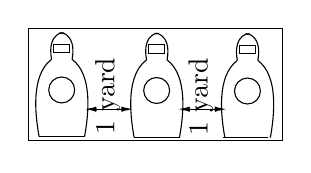
\begin{tikzpicture}[x=0.75pt,y=0.75pt,yscale=-0.25,xscale=0.25]
%uncomment if require: \path (0,300); %set diagram left start at 0, and has height of 300

%Curve Lines [id:da21318361798156604] 
\draw    (311.5,94) .. controls (301.5,40) and (340.5,41) .. (331,44) ;


%Curve Lines [id:da20785547955285444] 
\draw    (287.5,243) .. controls (279.5,199) and (271.5,124) .. (311.5,94) ;


%Curve Lines [id:da06117065871676419] 
\draw    (351.04,94) .. controls (361.04,40) and (321.5,41) .. (331,44) ;


%Curve Lines [id:da2984732943410131] 
\draw    (375.04,243) .. controls (383.04,199) and (391.04,124) .. (351.04,94) ;


%Straight Lines [id:da4437003370078836] 
\draw    (375.04,243) -- (287.5,243) ;


%Shape: Circle [id:dp7350896123282609] 
\draw   (306,153) .. controls (306,139.19) and (317.19,128) .. (331,128) .. controls (344.81,128) and (356,139.19) .. (356,153) .. controls (356,166.81) and (344.81,178) .. (331,178) .. controls (317.19,178) and (306,166.81) .. (306,153) -- cycle ;
%Shape: Rectangle [id:dp08228967328344328] 
\draw   (316,65) -- (346,65) -- (346,81) -- (316,81) -- cycle ;
%Curve Lines [id:da382305498912477] 
\draw    (486.5,95) .. controls (476.5,41) and (515.5,42) .. (506,45) ;


%Curve Lines [id:da4951194718210441] 
\draw    (462.5,244) .. controls (454.5,200) and (446.5,125) .. (486.5,95) ;


%Curve Lines [id:da6631408589263774] 
\draw    (526.04,95) .. controls (536.04,41) and (496.5,42) .. (506,45) ;


%Curve Lines [id:da1351424407246602] 
\draw    (550.04,244) .. controls (558.04,200) and (566.04,125) .. (526.04,95) ;


%Straight Lines [id:da4099829065086089] 
\draw    (546.04,244) -- (458.5,244) ;


%Shape: Circle [id:dp19778114222208343] 
\draw   (481,154) .. controls (481,140.19) and (492.19,129) .. (506,129) .. controls (519.81,129) and (531,140.19) .. (531,154) .. controls (531,167.81) and (519.81,179) .. (506,179) .. controls (492.19,179) and (481,167.81) .. (481,154) -- cycle ;
%Shape: Rectangle [id:dp30572188835967196] 
\draw   (491,66) -- (521,66) -- (521,82) -- (491,82) -- cycle ;
%Curve Lines [id:da34976216420835726] 
\draw    (128.5,93) .. controls (118.5,39) and (157.5,40) .. (148,43) ;


%Curve Lines [id:da22347635451446868] 
\draw    (104.5,242) .. controls (96.5,198) and (88.5,123) .. (128.5,93) ;


%Curve Lines [id:da4883303780747219] 
\draw    (168.04,93) .. controls (178.04,39) and (138.5,40) .. (148,43) ;


%Curve Lines [id:da4097889870486955] 
\draw    (192.04,242) .. controls (200.04,198) and (208.04,123) .. (168.04,93) ;


%Straight Lines [id:da32419947120502] 
\draw    (192.04,242) -- (104.5,242) ;


%Shape: Circle [id:dp3625259878314111] 
\draw   (123,152) .. controls (123,138.19) and (134.19,127) .. (148,127) .. controls (161.81,127) and (173,138.19) .. (173,152) .. controls (173,165.81) and (161.81,177) .. (148,177) .. controls (134.19,177) and (123,165.81) .. (123,152) -- cycle ;
%Shape: Rectangle [id:dp6927466091727594] 
\draw   (133,64) -- (163,64) -- (163,80) -- (133,80) -- cycle ;
%Straight Lines [id:da9164432991041944] 
\draw    (206,189) -- (272,189) ;
\draw [shift={(274,189)}, rotate = 180] [color={rgb, 255:red, 0; green, 0; blue, 0 }  ][line width=0.75]    (10.93,-3.29) .. controls (6.95,-1.4) and (3.31,-0.3) .. (0,0) .. controls (3.31,0.3) and (6.95,1.4) .. (10.93,3.29)   ;
\draw [shift={(204,189)}, rotate = 0] [color={rgb, 255:red, 0; green, 0; blue, 0 }  ][line width=0.75]    (10.93,-3.29) .. controls (6.95,-1.4) and (3.31,-0.3) .. (0,0) .. controls (3.31,0.3) and (6.95,1.4) .. (10.93,3.29)   ;
%Straight Lines [id:da11302707467047135] 
\draw    (386,189) -- (452,189) ;
\draw [shift={(454,189)}, rotate = 180] [color={rgb, 255:red, 0; green, 0; blue, 0 }  ][line width=0.75]    (10.93,-3.29) .. controls (6.95,-1.4) and (3.31,-0.3) .. (0,0) .. controls (3.31,0.3) and (6.95,1.4) .. (10.93,3.29)   ;
\draw [shift={(384,189)}, rotate = 0] [color={rgb, 255:red, 0; green, 0; blue, 0 }  ][line width=0.75]    (10.93,-3.29) .. controls (6.95,-1.4) and (3.31,-0.3) .. (0,0) .. controls (3.31,0.3) and (6.95,1.4) .. (10.93,3.29)   ;
%Shape: Rectangle [id:dp6077803871227272] 
\draw   (83.5,33) -- (573.5,33) -- (573.5,250) -- (83.5,250) -- cycle ;

% Text Node
\draw (236,164) node [rotate=-270] [align=left] {1 yard};
% Text Node
\draw (416,165) node [rotate=-270] [align=left] {1 yard};


\end{tikzpicture}

		\end{center}
				
		\\[0.6\textheight]
	\end{tabular}
	% Steps and Scoring	
	\begin{tabular}{ | p{0.65\textwidth} |}
		\hline
		%%%%%%%%%%%%%%%%%%%%%%%%%%%
		% Steps                   %
		%%%%%%%%%%%%%%%%%%%%%%%%%%%
		\rowcolor[HTML]{C0C0C0}Steps\\ 
		\hline
		\tiny \begin{enumerate}[topsep=0pt, partopsep=0pt]
			\item Starting on the left most target, place one shot on the left target.
			\item Place two shots on the center target.
			\item Place three shots on the right target.
			\item Place four shots on the center target.
			\item Place five shots on the left target.
		\end{enumerate}		
		\\ [0.25\textheight]
		\hline
		%%%%%%%%%%%%%%%%%%%%%%%%%%%
		% Scoring                 %
		%%%%%%%%%%%%%%%%%%%%%%%%%%%
		\rowcolor[HTML]{C0C0C0}Scoring \\
		\hline
		\tiny \begin{itemize}[topsep=0pt, partopsep=0pt]
			\item All shots should land within an 8" circle in the center mass of the targets. (5pts)
			\item For added challenge, all shots should land in a 3x5" index card in the center of the target. (10pts)
			\item Passing Hit Factor HF): 15.0
		\end{itemize}		
		\\ [0.25\textheight]
		\hline
	\end{tabular}
\end{document}
